\begin{frame}[label=current]
\frametitle{Euclidean Distance in Coordinates}
\begin{theorem}[Can be taken as definition]
The distance b-n the points $A(x_A,y_A,z_A)$ and $B(x_B,y_B,z_B)$ is given by:

$
\displaystyle d(A,B) = |AB| = \sqrt{(x_B-x_A)^2+(y_B-y_A)^2+(z_B-z_A)^2}
$
\end{theorem}
\begin{columns}
\column{0.3\textwidth}
\psset{xunit=0.7cm, yunit=0.7cm}
\begin{pspicture}(-2, -1)(2,2)
\renewcommand{\fcScreen}{[-0.5 1 -0.2] -1}
\tiny
\psline[linecolor=black!1](2, 4)(2, 4.01)
\fcAxesIIId{3}{3}{3}
\uncover<3->{
\fcPolyLineIIId[linecolor=red]{[2.6 1 1][2.6 1.4 1] [3 1.4 1] }
}
\uncover<4->{\fcPolyLineIIId[linecolor=red]{[2.8 3.7 1][2.8 3.7 1.360555128] [3 4 1.360555128] }}

\uncover<2->{\fcPolyLineIIId[linestyle=dotted]{ [1 1 1] [1 4 1] [1 4 3]}
\fcLineIIId[linestyle=dotted]{[1 4 1]}{[3 4 1]}
\fcParallelogramHollowIIId{ [1 1 1] }{ [3 1 1] }{ [3 1 3] }
\fcParallelogramHollowIIId{ [1 1 3] }{ [3 1 3] }{ [3 4 3] }
\fcParallelogramHollowIIId{ [3 1 1] }{ [3 4 1] }{ [3 4 3] }
}

\uncover<3->{\fcLineIIId[linestyle=dotted]{[1 1 1]}{[3 4 1]}}
\uncover<4->{\fcLineIIId[linestyle=dotted]{[1 1 1]}{[3 4 3]}}

\fcPutIIId[t]{[1 1 0.9]}{$A$}
\fcDotIIId[linecolor=black]{[1 1 1]}
\fcPutIIId[l]{[3 4 3]}{$~~B$}
\fcDotIIId[linecolor=black]{[3 4 3]}
\uncover<2->{
\fcPutIIId[l]{[3 4 1]}{$~~C$}
\fcPutIIId[t]{[3 1 0.9]}{$D$}
}
\uncover<6->{\fcPutIIId[t]{[2 1 0.9]}{\alert<6>{$x_B- x_A$}}}
\uncover<7->{\fcPutIIId[tl]{[3 2.5 1]}{\alert<7>{$~~y_B- y_A$}}}
\uncover<8->{\fcPutIIId[l]{[3 4 2]}{\alert<8>{$~~z_B- z_A$}}}
\end{pspicture}
\column{0.6\textwidth}
\uncover<2->{Why is this so? Geometric explanation:}
\[
\begin{array}{r@{}c@{}ll|l}
\uncover<3->{\alert<5>{|AC|^2} &~\alert<5>{=}~& \alert<5>{|AD|^2+|DC|^2} &&  \alert<3>{\triangle ADC}\\}
\uncover<4->{|AB|^2 &~=~&  |BC|^2+\alert<5>{|AC|^2}&& \alert<4>{ \triangle ACB}\\}
\uncover<5->{&~=~&|\alert<8>{BC}|^2+\alert<5>{|\alert<6>{AD}|^2+|\alert<7>{DC}|^2} \\}
\uncover<6->{&~=~&\phantom{+} (\alert<6>{x_B-x_A})^2+(\alert<7>{y_B-y_A})^2\\
&&+(\alert<8>{z_B-z_A} )^2\quad ,}
\end{array}
\]
\end{columns}

%\psfrag{O}{$O$}
%\psfrag{A}{$A$} 
%\psfrag{B}{$B(x_B, y_B, z_B)$}  
%\psfrag{C}{$C(x_B, y_B, z_A)$}    
%\psfrag{x}{$y$} 
%\psfrag{y}{$x$} 
%\psfrag{z}{$z$}     
%\psfrag{dx}{$y_B - y_A$}
%\psfrag{dy}{$x_B - x_A$}
%\psfrag{dz}{$z_B - z_A$}  
%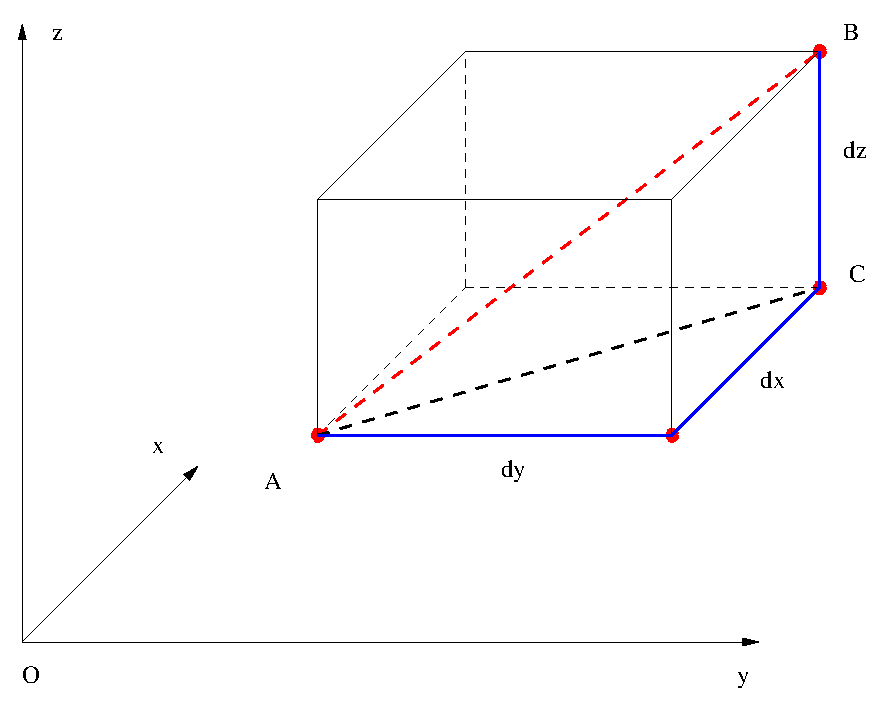
\includegraphics[height=1in]{../../modules/coordinate-systems/pictures/euclidean_distance.eps}
%
%
\uncover<9->{
Example: \[d(P(3,1,2), Q(1,2,3)) = \uncover<9>{\alert<9>{\textbf ?}} \uncover<10->{\alert<10>{{ \sqrt{(1-3)^2+(2-1)^2+(3-2)^2} = \sqrt{6} }}}\quad .\]
}

\end{frame}